\documentclass{beamer}
\usepackage[utf8]{inputenc}
\usepackage{listings}
\usepackage{multicol}
\usetheme{Berlin}
\setbeamercolor{palette secondary}{use=seahorse}
\usecolortheme{seahorse}
\title[How to be a Vim Ninja]{How to be a Vim Ninja}
\author{\hspace{12pt}Robert “Anthony” Bittle\hspace{12pt}\\\hspace{12pt}robert.bittle@dominionenterprises.com\hspace{12pt}\\\hspace{12pt}github.com/guywithnose\hspace{12pt}}
\date{December 15, 2014}
\setbeamertemplate{itemize items}[circle]
\begin{document}
    \begin{frame}
        \titlepage
        Slides and demos at:\\
        \href{https://github.com/guywithnose/de-devcon-vim}{https://github.com/guywithnose/de-devcon-vim}\\
        \href{http://bit.ly/11po3hk}{http://bit.ly/11po3hk}
    \end{frame}

    \section{Intro}
    % \begin{frame}{Who am I?}
    %     \begin{itemize}
    %         % Be quick, maybe cut this slide
    %         \item robert.bittle@dominionenterprises.com
    %         \item github.com/guywithnose
    %     \end{itemize}
    % \end{frame}

    % Find out where the audience is
    % Have you ever used vim before
    % Do you only use it when you are composing git commit messages?
    % Do you use it regularly?
    % Is it your primary editor?
    \subsection{Why Vim?}
    \begin{frame}{Why is Vim hard to learn?}
        \begin{itemize}
            \item Vim is extremely complex % This is a pro and a con
            \item Vim is full of features that are not imediately discoverable
            \item Vim is designed for experienced developers not beginners.
        \end{itemize}
        % It takes time to learn the complexity, but over time you learn the
        % commands and eventually it is all muscle memory.
    \end{frame}
    \begin{frame}{Why is Vim worth the steep learning curve?}
        \begin{itemize}
            \item Vim is designed to maximize your productivity potential.
            \item Vim can automate the tedious tasks so that text editing doesn't get in the way of coding.
        \end{itemize}
        % Vim does a little bit to get you started, but it really can be a pain
        % to beginners.  Learning vim is often done through community.  The
        % best reason to learn vim is because you've seen someone you know use
        % it properly.  One of the best motivations to learn vim is know how
        % well you saw someone else use it.  It may take a while.
    \end{frame}
    \begin{frame}{The power of modes}
        \begin{figure}
            \centering
            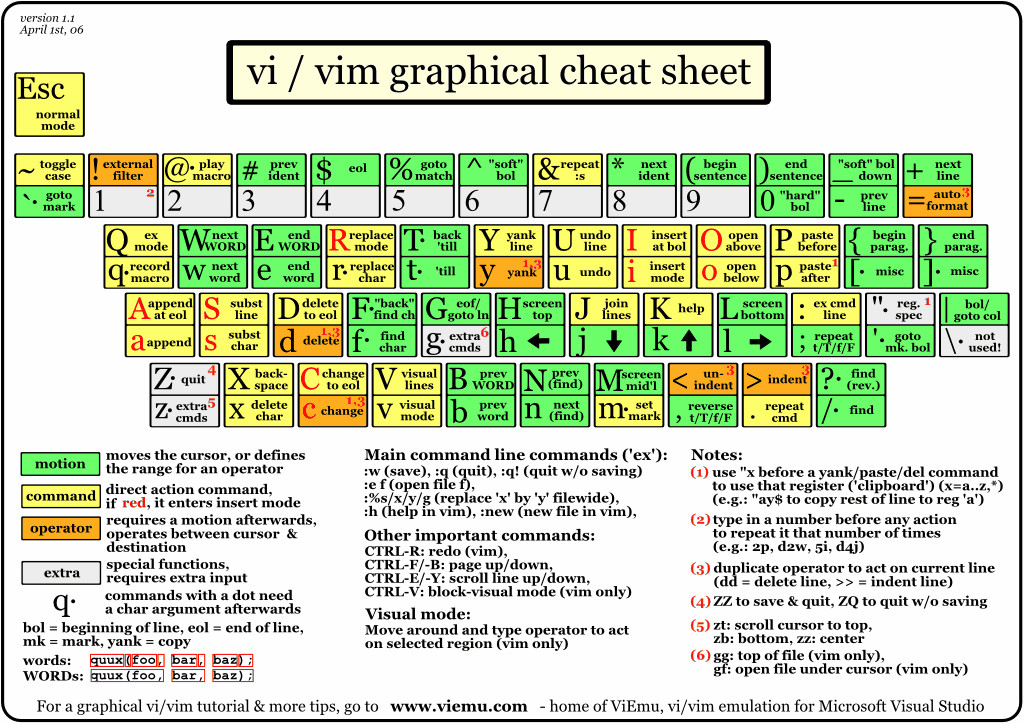
\includegraphics[width=0.8\linewidth]{vi-vim-cheat-sheet.jpg}
        \end{figure}
        % Vim is able to have so many features because in normal mode
        % all of the keyboard is free for shortcuts.
    \end{frame}
    % \subsection{The power of Vim}
    % Since I want to aim this talk at intermediate vim users this might be
    % unnecessary.  It may be worth leaving if we bring in the :move command.
    % Either way we should talk about how using the mouse can slow you down.
    %
    % \defverbatim[colored]\lstLinesFlipped{
    %     \begin{lstlisting}
% Second line.
% First line.
    %     \end{lstlisting}
    % }
    % \defverbatim[colored]\lstArrow{
    %     \begin{lstlisting}
% -------->
    %     \end{lstlisting}
    % }
    % \defverbatim[colored]\lstLinesCorrect{
    %     \begin{lstlisting}
% First line.
% Second line.
    %     \end{lstlisting}
    % }
    % \begin{frame}{Moving text}{What we want to do}
    %     \begin{multicols}{3}
    %         \lstLinesFlipped
    %         \columnbreak
    %         \pause
    %         \lstArrow
    %         \columnbreak
    %         \lstLinesCorrect
    %     \end{multicols}
    % \end{frame}
    % \begin{frame}{Moving text}{How we can do it}
    %     \begin{itemize}
    %         \item <alert@+> Standard text editor
    %         \begin{itemize}
    %             % Using mouse
    %             \item <alert@+> Highlight with mouse and drag
    %             \item <alert@+> Highlight with mouse, Ctrl-x, Down, Ctrl-v
    %             \item <alert@+> Home, Shift-Down, Ctrl-x, Down, Ctrl-v (8 keystrokes)
    %         \end{itemize}
    %         \item <alert@+> Vim
    %         \begin{itemize}
    %             \item <alert@+> dd(Cut a line)p(Paste) (3 keystrokes)
    %         \end{itemize}
    %    \end{itemize}
    % \end{frame}
    \section{How to learn Vim}
    % I only have an hour today, so I can only scratch the surface of vim's
    % capabilities and lets be honest if I only show you a few things that I
    % think are cool you might remember 10% of this. Instead I want to point
    % you in the right direction and teach you how to learn vim because vim is
    % best learned over time.  The only way I know how to master vim is by
    % learning a small number of things at a time over a long period of time.
    \subsection{}
    % \begin{frame}{Learn the basic commands}
    %     \begin{itemize}
    %         \item <alert@+> vimtutor
    %         \item <alert@+> Vim documentation
    %     \end{itemize}
    % \end{frame}
    \begin{frame}{vimtutor}
        \begin{itemize}
            \item vimtutor is a primer for the base functionality, but it is only enough to get you started.
            \item The most important thing you learn in vimtutor is where to find the manual.
        \end{itemize}
    \end{frame}
    \begin{frame}{Vim documentation}
        \begin{itemize}
            \item Vim has very exhaustive documentation.
            \item It is not intended to be read completely.  % 6MB of text
            \item Learn to use the search functionality (:helpgrep).
                % This is a great place to demonstrate where to find vim
                % documentation, how to search it and how to navigate it.
                %
                % Also mention that if vim doesn't do what you are looking for
                % natively, you might be able to find a plugin for it.
                %
                % Open a vim terminal and talk about a common mistake of
                % transposing :q.  Explain how this error can be seen as an
                % annoyance or as a learning opportunity.  :h q:
                %
                % commandLineWindow.txt
                % Show how the command line window can be very powerful.  The
                % command history can be traversed with the <up> <down> keys,
                % but the command line window can be searched.  Think about
                % what it means to search your searches.  Change master to
                % grok.
                %
                % Open help for /
                % :helpgrep spell check
        \end{itemize}
    \end{frame}
    \begin{frame}{Maintain a cheatsheet}
        \begin{itemize}
            \item Decide on a few (no more than 10) things you want to learn.
            \item Write them down where you can see them while you are working in vim.
            \item Force yourself to use them in real world scenarios.
                % If you do something and then realize you could have used what
                % you are learning, undo and use the new technique.  If you
                % never run into a real world scenario to use a cool feature of
                % vim, then erase it from your list and don't waste your time
                % learning it.
        \end{itemize}
    \end{frame}
    \section{Macros}
    \subsection{}
    % To really maximize the potential of vim, you need to learn to recognize
    % when you are frequently doing the same mechanical operations.  Macros
    % allow you to record these operations and then play them back.  It is
    % clear to see how this would save you keystrokes, but recording the macro
    % in a repeatable way can be tricky.
    \begin{frame}{Recognize mechanical operations}
        \begin{itemize}
            \item How often do I do this?
            \item How long did it take me?
            \item Can it be scripted?
        \end{itemize}
    \end{frame}
    \begin{frame}{Basic commands}
        \begin{itemize}
            \item q[0-9a-z] - start recording
            \item Do something that is repeatable
            \item q - stop recording
            \item @[0-9a-z]
            \item :help complex-repeat
        \end{itemize}
    \end{frame}
    \begin{frame}{Tips}
        \begin{itemize}
            \item Try to start the macro with an operation that will fail after the last iteration.
            \item Try to avoid absolute motions.
            \item Use search motions, word motions, mark motions, etc.
        \end{itemize}
        % This definitely calls for a demo.  Create a file just for this
        % demonstration with the macros spelled out.  Maybe even include a
        % naive example and show why it doesn't work. Maybe wrap a bunch of
        % lines in an html tag.
        %
        % macros.js
    \end{frame}
    \section{Level up your .vimrc}
    \subsection{}
    \begin{frame}{What is a vimrc file?}
        \begin{itemize}
            \item Your vimrc file is where you store your custom vim configuration.
            \item Vim loads this information every time that it starts up.
                % So be careful not to add a lot of bloated plugins
            \item As you become a more mature vim user, your vimrc will grow to include all the special sauce that makes vim work the way you like it.
        \end{itemize}
    \end{frame}
    \begin{frame}{Mappings}
        \begin{itemize}
            \item Mappings are an easy way to bind macros to a key or combination of keys.
                % Talk about leader commands
            \item Over time as you find ways to automate common operations with macros you can save them as mappings in you vimrc file.
                % Demonstrate how to paste a recorded macro as a mapping
        \end{itemize}
    \end{frame}
    \section{Advanced techniques}
    \subsection{}
    \begin{frame}{Motions and Actions (Vim grammar)}
        Actions
        \begin{itemize}
            \item Delete - d
            \item Change - c
            \item Yank (Copy) - y
        \end{itemize}
        Prepositions
        \begin{itemize}
            \item in - i
            \item around - a
        \end{itemize}
        Motions
        \begin{itemize}
            \item Word motions -- w, W, b, B, e, ge, E, gE
            \item Search motions -- t, T, f, F, /
            \item Text object motions -- p, s, \}, ], ), $>$, ', "
        \end{itemize}
    \end{frame}
    \begin{frame}{Dot Command}
        % A good demo is replacing a local variable with a class variable in PHP.
        % ciwthis->foojj.
        Repeat last action
        \begin{itemize}
            \item Think of this like an automatic mini macro.
            \item Combine simple actions using the change(c) action.
        \end{itemize}
    \end{frame}
    \begin{frame}{Autocomplete}
        \begin{itemize}
            \item Ctrl-P
            \item Ctrl-N
            \item Ctrl-X Ctrl-L
            \item Ctrl-X Ctrl-F
            \item Ctrl-X Ctrl-O
        \end{itemize}
    \end{frame}
    \section{Plugins}
    \subsection{}
    \begin{frame}{How to install plugins}{Pathogen}
        \begin{itemize}
            \item Add pathogen.vim to \textasciitilde/.vim/autoload
            \item Add this line to your .vimrc\\
                \quad execute pathogen\#infect()
            \item Plugins get loaded from \textasciitilde/.vim/bundle
        \end{itemize}
    \end{frame}
    \begin{frame}{How to install plugins}{Git}
        Once you have Pathogen installed
        \begin{itemize}
            \item Copy plugins to your bundle directory.
            \item If the plugin is in git you can check it out to a directory in bundle.
            \item Take advantage of git submodules.
                % This is really useful if you like to keep your settings
                % synchronized across two systems.
        \end{itemize}
    \end{frame}
    % Before introducing this, demonstrate what a mechanical operation is by
    % showing the motivation behind split-join
    \subsection{Crafting your own plugins}
    \begin{frame}{Directory structure}
        \begin{itemize}
            \item plugin
            \item ftplugin
            \item autoload
            \item doc
        \end{itemize}
    \end{frame}
    % A word about plugins:
    % Get to know the base functionality first.  Many plugins extend or change
    % current functionality and add or overwrite key commands.  Make sure you
    % know what you are giving up for a plugin.  It may be better to use built
    % in functionality.  Keep in mind that every plugin you add can potentially
    % slow down vim's load time.  With that said, here a few of my favorites.
    \begin{frame}{My Favorite Plugins}
        \begin{itemize}
            \item Editing tasks
                \begin{itemize}
                    \item Surround
                    \item Ultisnips
                \end{itemize}
            \item Folding (Usually language specific)
            \item Interface
                \begin{itemize}
                    \item fugitive
                    \item CtrlP
                \end{itemize}
        \end{itemize}
    \end{frame}
\end{document}
